\section{Evaluation}
\label{sec:evaluation}
This section describes our evaluation methodology and results.
These evaluations assume a 3 GHz clock, which is a typical CPU clock speed.

\begin{figure*}
  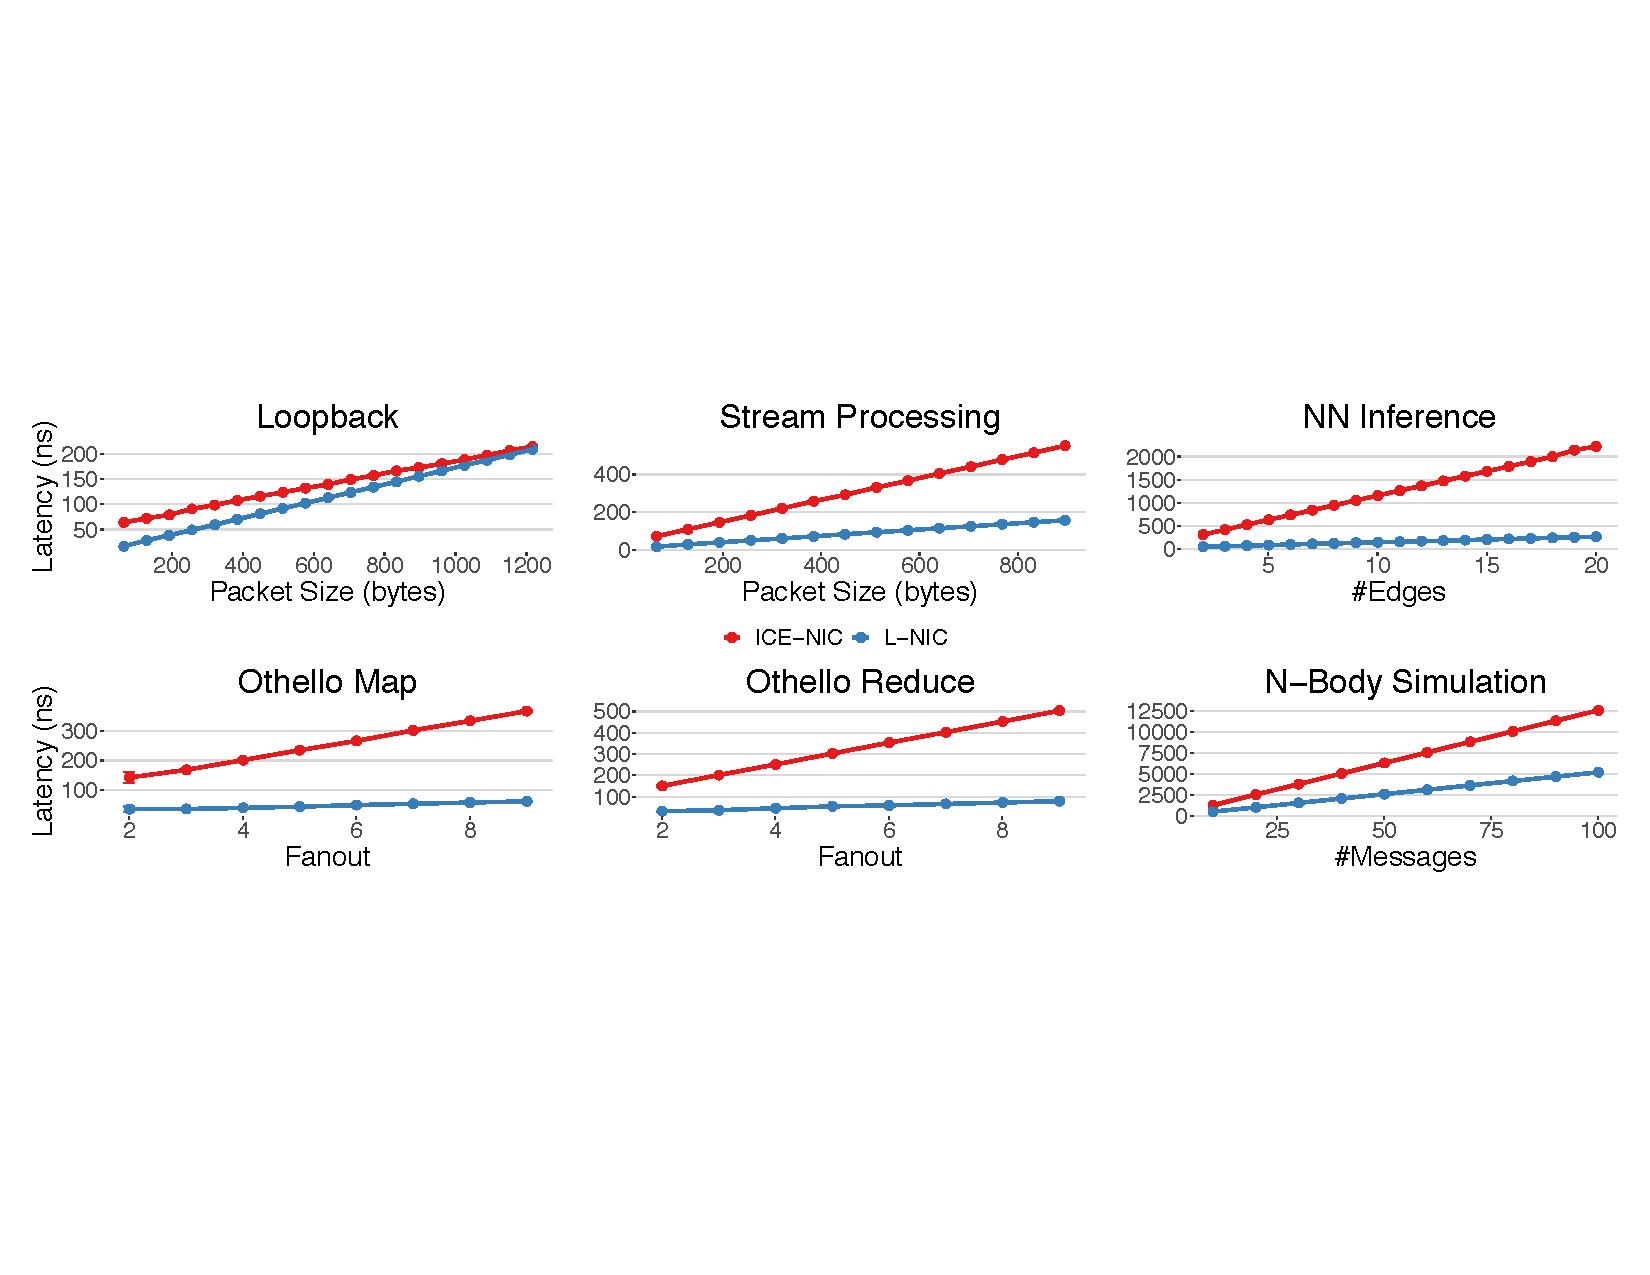
\includegraphics[width=\linewidth]{./figures/latency}
  \caption{Nanoservice application latency comparisons for \name{} vs a traditional RISC-V core with IceNIC.}
  \label{fig:latency}
\end{figure*}

\steve{change IceNIC label to RISC-V w/ IceNIC and change L-NIC label to \name{} in Figure~\ref{fig:latency}}

\subsection{Microbenchmarks}
This section describes a set of microbenchmarks that characterize various aspects of the \name{} architecture.

\paragraph{Timing Analysis.} We synthesized both our \name{} RISC-V prototype as well as a standard RISC-V core with a traditional NIC (IceNIC) to a modern FPGA (Xilinx Ultrascale+) in order to analyze the critical paths in each design.
We found that the critical path in both designs is in the L2 cache, and hence our \name{} prototype is able to achieve the same clock rate as a traditional RISC-V system.

\paragraph{Basic Latency/Throughput Performance Analysis.} The latency of the \name{}'s TX path is 11 cycles for a single word message, which is measured from the cycle when an application writes the word to when the word is placed on the network (not including the MAC processing).
The corresponding latency of the RX path is 6 cycles.
These latency measurements do not include MAC processing.
Figure~\ref{fig:latency} shows the loopback latency for various packet lengths for both our \name{} prototype and the traditional DMA-based IceNIC.
The \name{} provides about a 4$\times$ latency reduction for small packets and a much smaller speedup for large packets due to the store-and-foreword nature of the current \name{} prototype's TX path.
In the case of IceNIC, the CPU is mostly idle during these simple loopback experiments because it only needs to instruct the NIC's DMA engine to send/receive packets and to swap source an destination header fields.
However, in the case of the \name{}, the CPU is fully utilized because it touches every byte of every packet.

Table\ref{tab:throughput} shows the TX and RX throughput for 64B packets for both our \name{} prototype and RISC-V with IceNIC.
The \name{} is able to achieve 6-8$\times$ higher throughput than the traditional network interface.
This performance gain is mainly a result of the significantly reduced per-packet overheads in the \name{}.
A \name{} application does not need to instruct a DMA engine to send/receive packets, it simply reads and writes the NIC queues directly.

\begin{table}
\begin{center}
\begin{tabular}{|c|c|c|}
\hline
                          & \textbf{RX (Gbps)} & \textbf{TX (Gbps)} \\ \hline
\textbf{\name{}}          & 116                & 186                           \\ \hline
\textbf{RISC-V w/ IceNIC} & 14                 & 28                            \\ \hline
\end{tabular}
\caption{TX and RX throughput achievable by both our \name{} prototype and a traditional RISC-V core with IceNIC for 64B packets.}
\label{tab:throughput}
\end{center}
\end{table}

%\begin{figure}
%  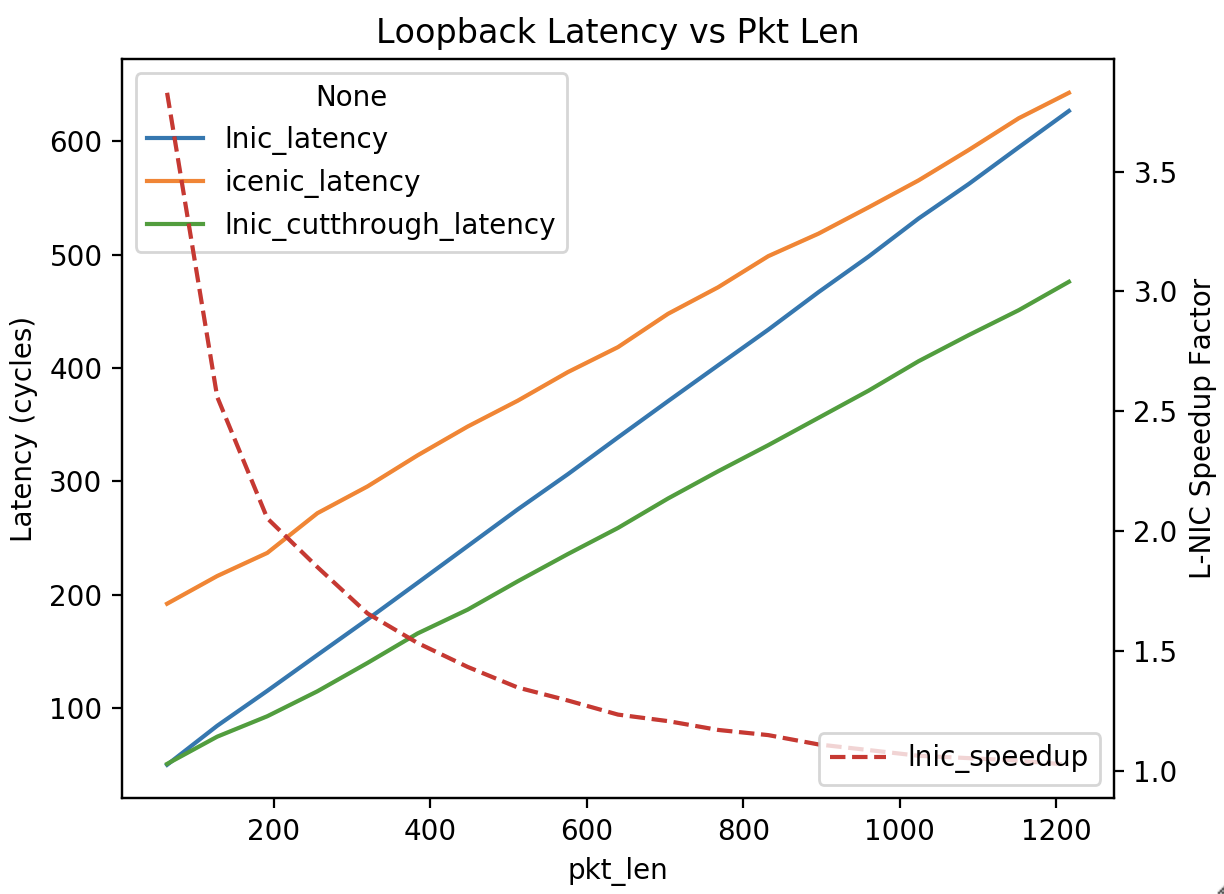
\includegraphics[width=\linewidth]{./figures/loopback-latency}
%  \caption{\name{} vs Traditional net-core-net loopback latency for various packet sizes.}
%  \label{fig:loopback-latency}
%\end{figure}

\paragraph{nanoKernel Scheduler Latency.} We measure the latency of the nanoKernel scheduler as the time from when an interrupt fires to the time when the first instruction of the newly selected thread is executed.
We find that the nanoKernel scheduler latency is \SI{60}{ns} (180 clock cycles).
\steve{How does this compare to the latency of modern schedulers?}

\subsection{Bare Metal Application Evaluations}
\label{ssec:bare-metal-evals}
This section describes the reduction in average latency as a result of the \name{}'s hardware fast path to the core of the CPU.
For our evaluations we consider 4 example nanoservice applications, each of which are implemented as bare metal apps on top of both our \name{} prototype and a traditional IceNIC-based processor.

\paragraph{NFV Style Streaming Application.} This simple application treats the arriving message as a list of 8 byte unsigned integers and increments each integer then returns the resulting message back to the sender.
The latency is measured from the time when the first byte of the request enters the NIC to when the last byte of the response leaves the NIC.
The \name{} is able to achieve a 3.5-4$\times$ speedup over the IceNIC system across all packet lengths, as shown in Figure~\ref{fig:latency}.

The most significant difference between this application and the loopback application is that the CPU is forced to touch every byte of every packet.
This means that for the IceNIC implementation, every byte of the packet must be copied from memory into registers, sent through the ALU, and then copied back into memory before the DMA engine can send out the final packet.
These operations lead to a lot of overhead and extra latency for IceNIC, none of which exist for the \name{} because it never needs to touch memory.

% Note that this type of application meets the criteria outlined in Section XXX to be considered a nanoservice application.
% Each message is processed independently, so it is highly parallelizable.
% Since NFV applications typically need to process messages as fast as possible, it is reasonable to expect that they will want to process each message within a microsecond.
% The simple example of an NFV style streaming application evaluated here is stateless between packets and hence the working set only needs to be large enough for the local computation, which in this case, is small enough to reside in the register file and never touches memory at all.
% Other NFV applications such as firewalls or intrusion detection systems would have a larger working set, especially if they need to match against a large list of rules.
% As long as this working set is cache resident, the application can be considered a nanoservice.

%\begin{figure}
%  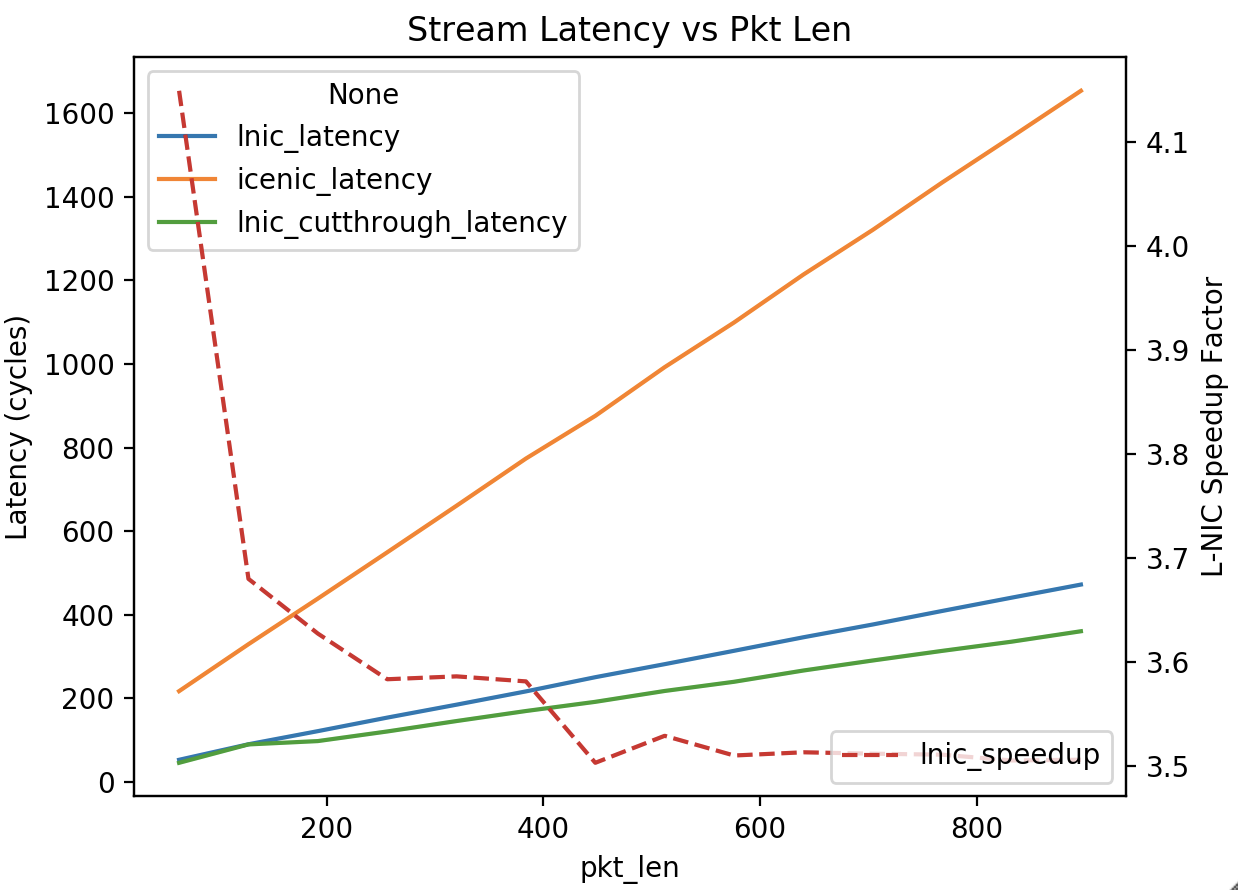
\includegraphics[width=\linewidth]{./figures/stream-latency}
%  \caption{\name{} vs Traditional NFV-style streaming application latency for various packet sizes.}
%  \label{fig:stream-latency}
%\end{figure}

\paragraph{Neural Network Inference.} This application can be implemented using nanoservice where each node of the neural network is running on a separate \name{} core.
This exploits the maximum amount of model parallelism,  minimizing the latency required to perform an inference task.
Since the computation required by each node is essentially a running multiply-accumulate operation, it is reasonable to expect that the working set and message processing time will easily satisfy the constraints required to be considered a nanoservice.
Especially if the weights and data use reduced precision integers, as is typical in today's inference tasks~\cite{nn-quantization}.

We demonstrate this application by implementing the multiply-accumulate operation for a single node in a neural network.
The node receives $N$ weight messages and $N$ data messages, one for each incoming edge, then multiplies the corresponding data and weights and accumulates the result.
When all messages have been processed it sends a response message with the final result.
The latency is measured from the first byte of the first incoming message to the last byte of the response.
Figure~\ref{fig:latency} shows that the \name{} implementation is able to achieve about an order of magnitude latency reduction over the traditional IceNIC hardware.
The main reasons for the \name{}'s performance improvement are twofold: (1) Packet data does not need to be copied into registers before using the ALU, and (2) \name{} has a much higher RX throughput for small packets (as shown in Table~\ref{tab:throughput}).

%\begin{figure}
%  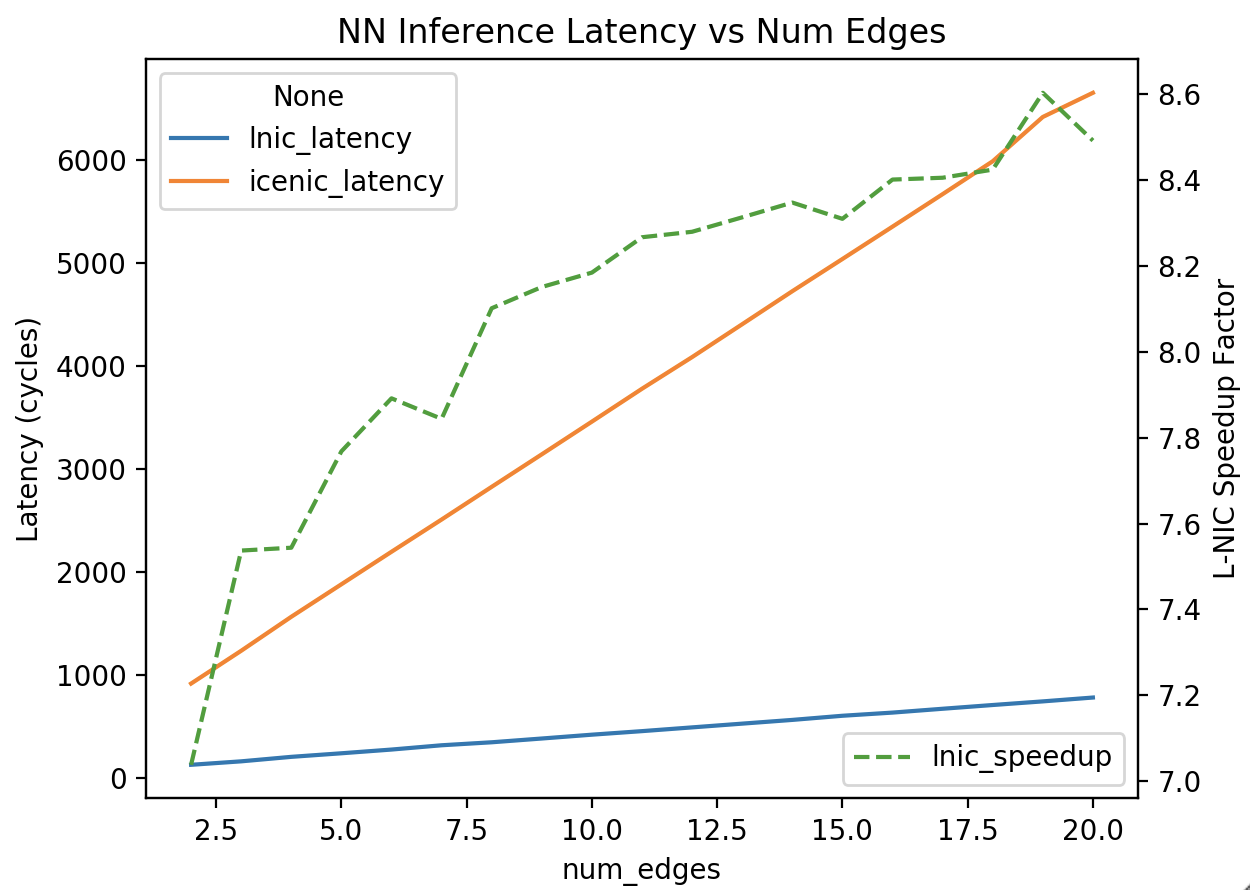
\includegraphics[width=\linewidth]{./figures/nn-inference-latency}
%  \caption{\name{} vs Traditional neural network node latency for various number of incoming edges.}
%  \label{fig:nn-latency}
%\end{figure}

\paragraph{Othello Map/Reduce.} We re-implemented the Othello application (as described in \cite{lnic}), comparing its performance on the \name{} with a traditional RISC-V core and IceNIC.
An Othello board can be represented using BitBoards~\cite{bitboard} with just two 64-bit unsigned integers and hence the working set of the nanotasks are all L1 cache resident.
The set of possible next moves can be calculated in less than one microsecond, as demonstrated in \cite{lnic}.

We measured the latency of the "map" and "reduce" functions as a function of the {\em fanout}, which is the number of possible next moves given an initial board state.
Because of the very short execution latency and the \name{}'s superior TX/RX throughput, the \name{} reduces the time for both functions by a factor of $4-6\times$, as shown in Figure~\ref{fig:latency}.

%\begin{figure}
%  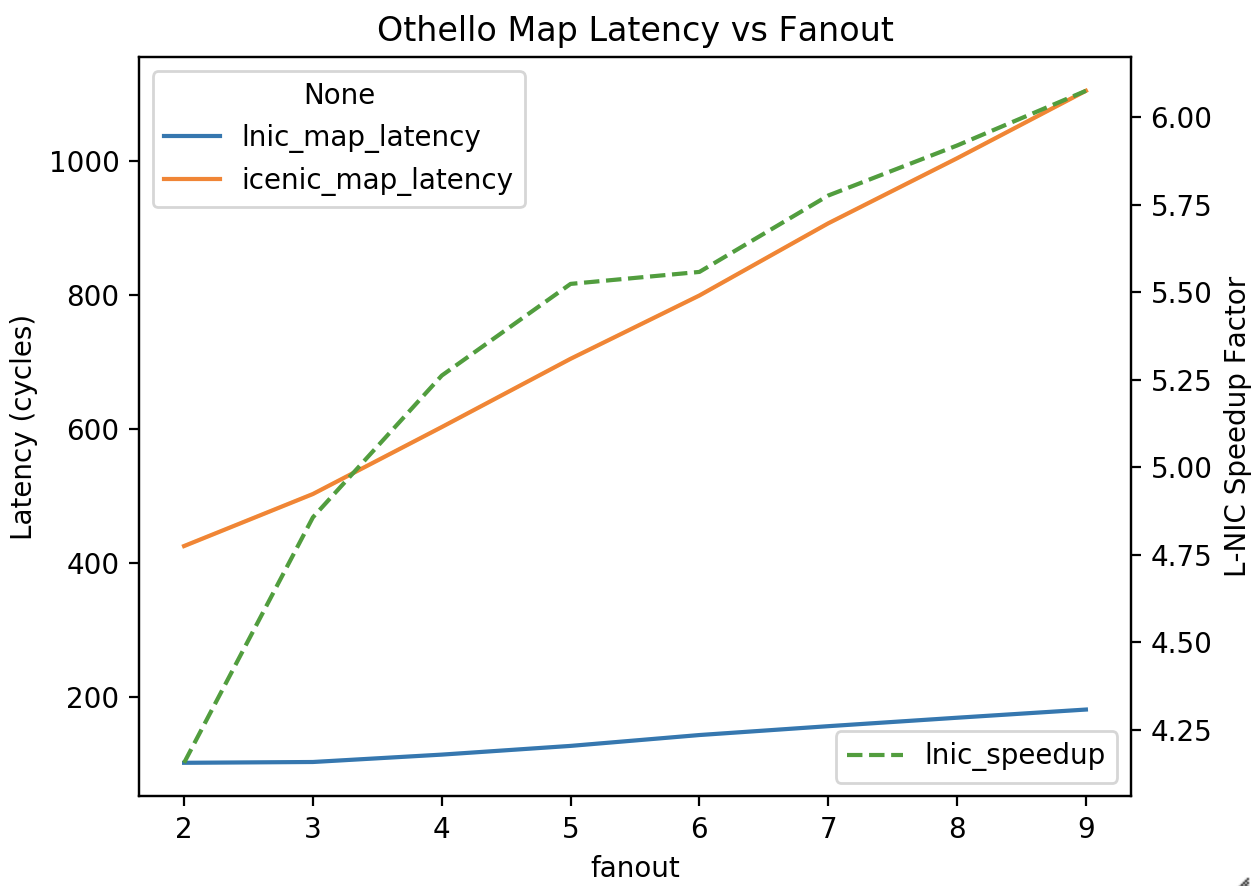
\includegraphics[width=\linewidth]{./figures/othello-map-latency}
%  \caption{\name{} vs Traditional Othello map latency for various degrees of fanout.}
%  \label{fig:othello-map-latency}
%\end{figure}
%
%\begin{figure}
%  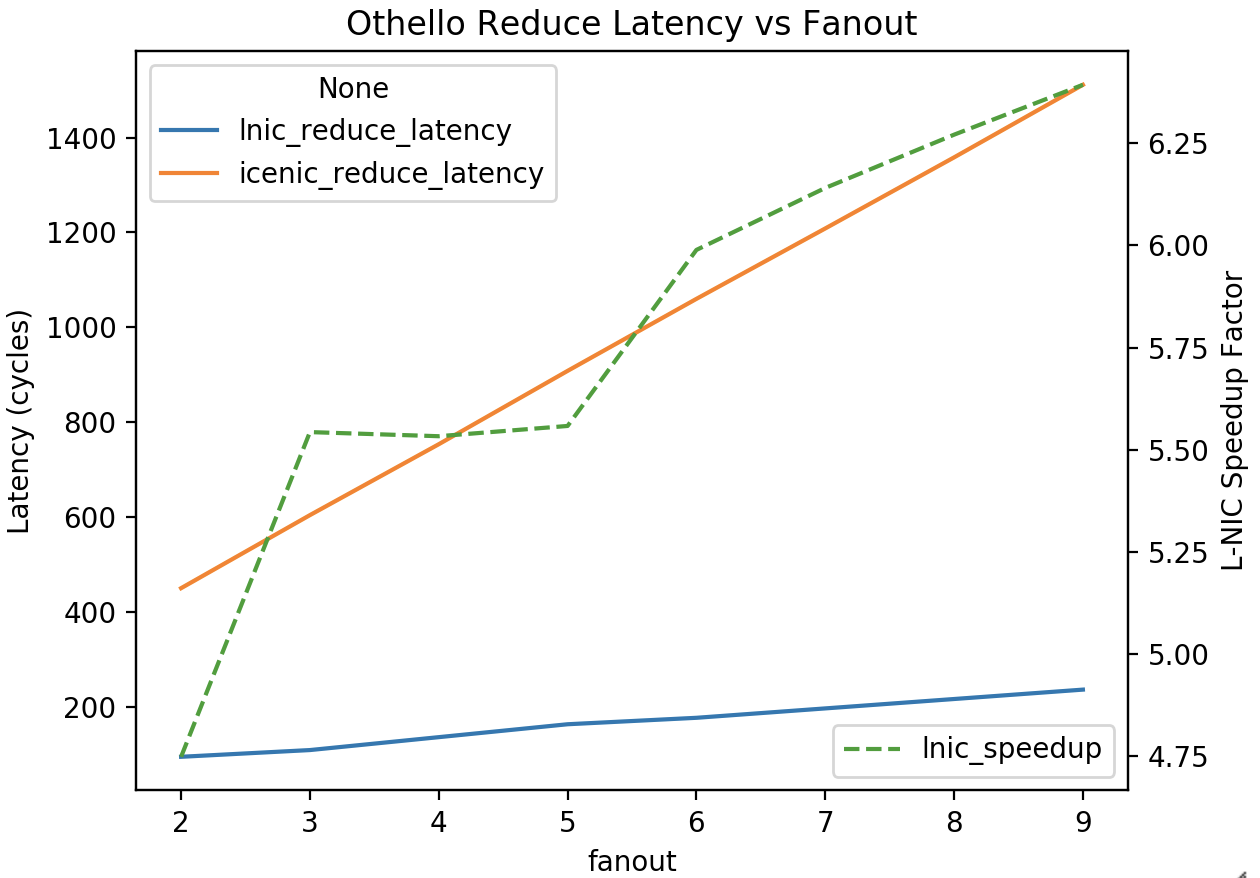
\includegraphics[width=\linewidth]{./figures/othello-reduce-latency}
%  \caption{\name{} vs Traditional Othello reduce latency for various degrees of fanout.}
%  \label{fig:othello-reduce-latency}
%\end{figure}

\paragraph{N-body Simulation.} This large class of applications is extremely well-suited to implementation using nanoservices.
An N-body simulation is a type of physical simulation commonly used in scientific computing and is typically run on HPC clusters.
Astronomers uses N-body simulations to model the gravitational interaction of celestial bodies.
These simulations are very computationally heavy, especially the steps that compute the gravitational force each body exerts on every other body.
A commonly used data structure for implementing an N-body simulation is a quad-tree, as described in the Barnes-Hut algorithm~\cite{barnes-hut}.
This algorithm reduces the computational complexity required for the gravity computation step from $O(N^2)$ to $O(\log N)$.
A naive nanoservices implementation of the Barnes Hut algorithm would simply implement each node of the quad tree as a separate nanotask.
In this case, the state required by each node is very minimal as it mainly consists of the node's position and mass, which is easily cache resident.
The computation required by each node consists of computing the force that the node exerts on the body indicated in the arriving message, which requires an evaluation of the following equation:
$$ F_G = G\frac{m_1 \cdot m_2}{r^2} $$
Where, $G$ is the gravitational constant, $m_1$ and $m_2$ are the masses of the two bodies, and $r$ is the distance between them.
Thus, the computation only requires a few floating point operations and the response time for each message is easily sub-microsecond.

We implemented a single node of an N-body physical simulation to evaluate the performance gain provided by the \name{}.
The node receives $N$ update messages which indicate the position of each body, and then evaluates the equation shown above to compute the gravitational force.
The result is included in a response message that is sent back into the network.
Latency is measured from when the first byte of the first request message enters the NIC to when the last byte of the last response message leaves the NIC.
As shown in Figure~\ref{fig:latency}, the \name{} provides a $2.5\times$ latency reduction over the traditional IceNIC system.

%\begin{figure}
%  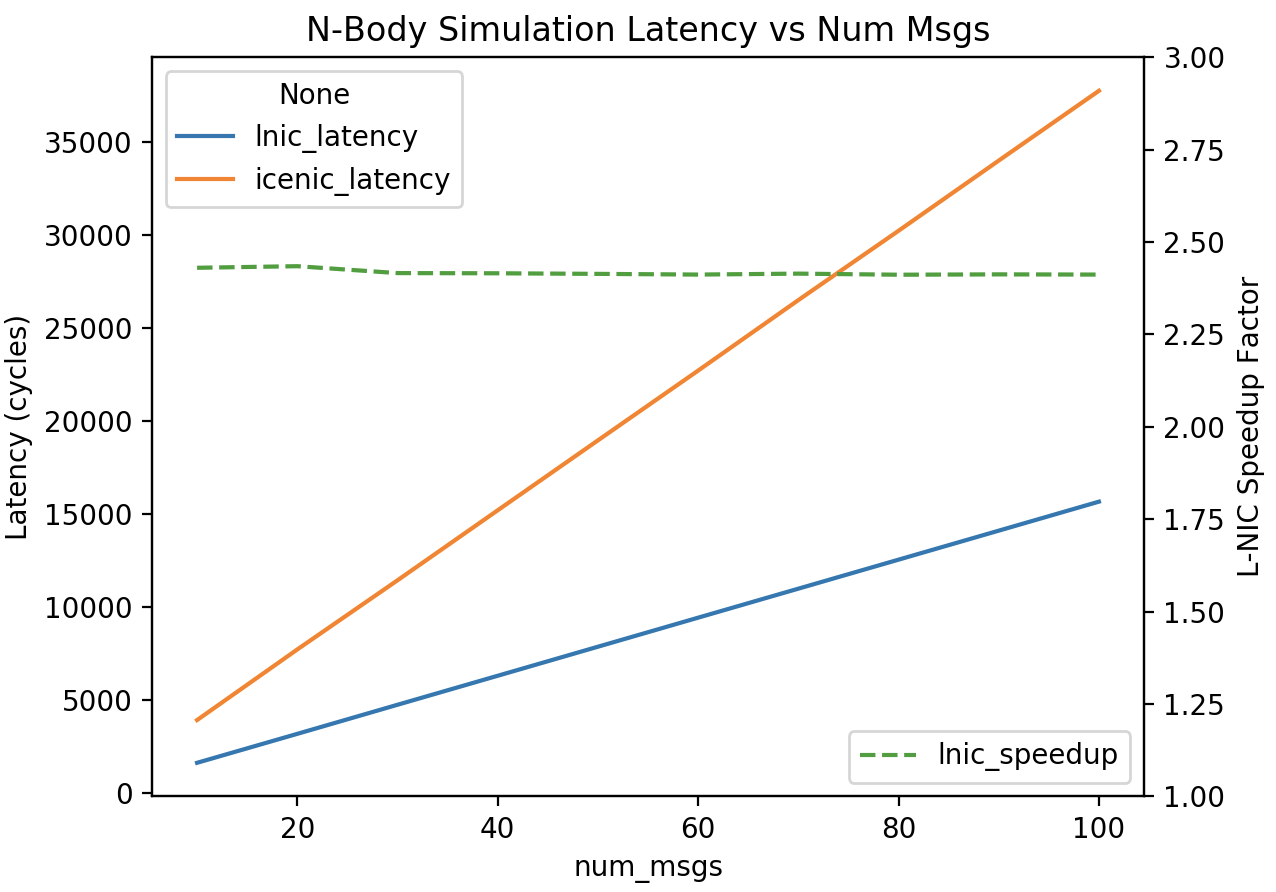
\includegraphics[width=\linewidth]{./figures/nbody-latency}
%  \caption{\name{} vs Traditional N-body simulation node latency.}
%  \label{fig:nbody-latency}
%\end{figure}

\subsection{Thread Scheduling Evaluations}
This section demonstrates the reduction in tail latency as a result of the NIC-driven thread scheduling policy used in our \name{} prototype.
We compare our NIC-driven thread scheduling policy, which was described in \S\ref{ssec:thread-scheduler}, to a more traditional Linux-style, timer driven thread scheduling approach.
In the timer-driven thread scheduling approach, timer interrupts are configured to fire periodically and NIC interrupts are disabled.
When an interrupt fires, the processor traps into the nanoKernel which then swaps to the context indicated by the NIC (i.e. the highest priority context with messages to process).
The key difference between the NIC-driven thread scheduling and the timer-driven thread scheduling approach is that in the later, context switches can only happen on periodic time boundaries.

We evaluate these scheduling policies by pinning one high priority context and one low priority context on the core, then sending in a stream of randomly interleaved high and low priority requests.
Each application will service the request for 500 ns then send back a response.
The inter packet gap of arriving messages is also configured to be about 500 ns.
Figure~\ref{fig:scheduling-latency} shows the distribution of response times for the high priority messages for both scheduling policies.
We see that NIC-driven scheduling reduces the tail response latency by a factor of about $5.5\times$ and the standard deviation of the response times is reduced by almost $20\times$.
This result should not be surprising because the NIC-driven scheduling policy is able to immediately evict the low priority thread once a high priority message arrives, whereas the timer-driven policy must wait for a timer interrupt.
Furthermore, we also measure that the NIC-driven scheduling policy is able to achieve slightly higher throughput for the low priority application.
This is because the timer-driven policy causes many traps into the nanoKernel for no reason, degrading its throughput.

We expect that both of these scheduler implementations are substantial improvements over what is commonly used in today's systems because they both use scheduling decisions made by the NIC hardware, whereas scheduling decisions in modern systems are made by slow software.
The purpose of this evaluation is simply to demonstrate the benefit of allowing the NIC to drive the context switch logic.

\begin{figure}
  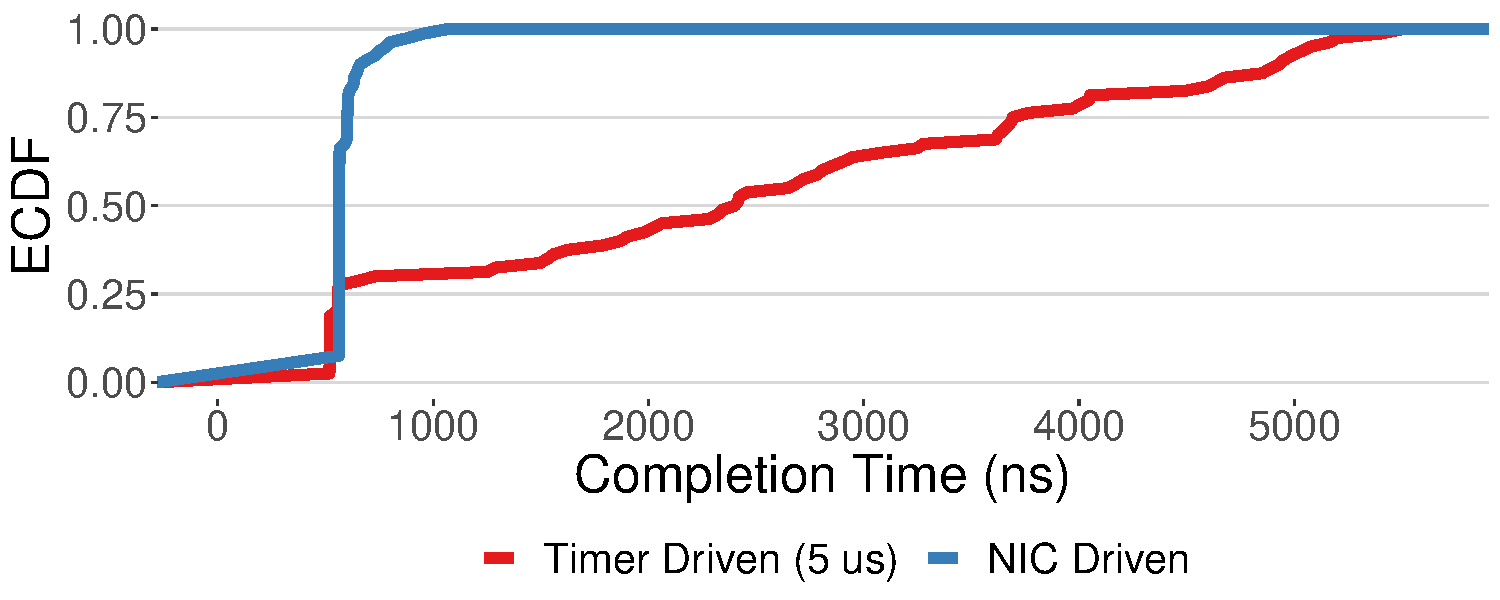
\includegraphics[width=\linewidth]{./figures/scheduling-comptimes}
  \caption{Latency reduction as a result of NIC-driven thread scheduling relative to timer-driven thread scheduling.}
  \label{fig:scheduling-latency}
\end{figure}

%\begin{figure}
%  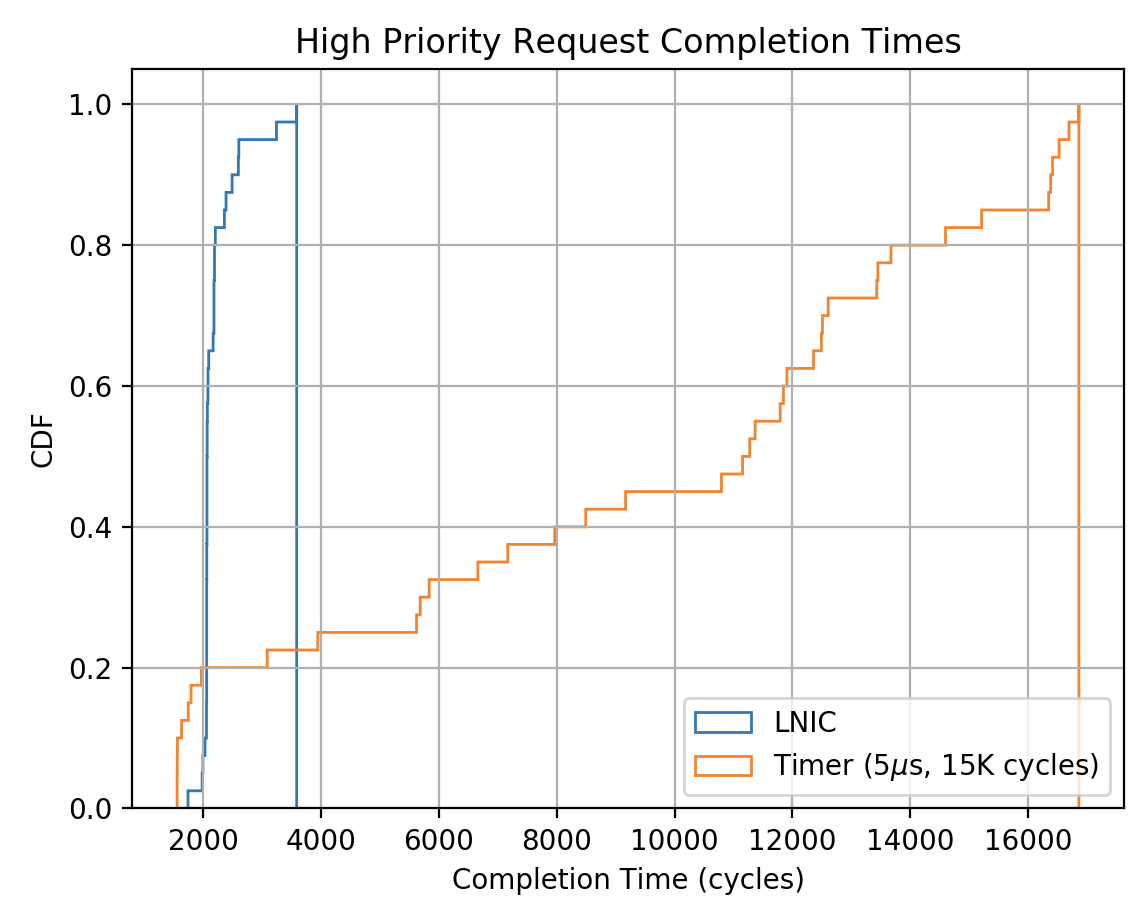
\includegraphics[width=\linewidth]{./figures/scheduling-tail-latency}
%  \caption{Latency reduction as a result of NIC-driven thread scheduling relative to timer-driven thread scheduling.}
%  \label{fig:scheduling-latency}
%\end{figure}

\subsection{Large Scale Nanoservice Evaluation}
In order to demonstrate the expected performance gains of a large scale nanoservice deployment we will use the N-body simulation application and the naive nanoservice implementation described in \S\ref{ssec:bare-metal-evals}.
Using this approach, the root node of the quad tree becomes the bottleneck, because it must process one message from each body being simulated.
In this case, the root node dictates the total runtime of the gravity computation.
We compare the theoretical performance of this naive nanoservice application with the performance obtained by using a commonly used N-body gravitational simulator, ChanGa~\cite{changa}.
Table~\ref{tab:nbody-changa} shows the average gravity computation time for 80K bodies using both the ChanGa simulator (with recommended parameter settings) and the naive nanoservices implementation.
We obtain the expected nanoservice performance by extrapolating the performance of the bare metal application N-body node, evaluated in \S\ref{ssec:bare-metal-evals}, to 80K messages.
This mimics the processing required by the root node of the quad tree.
We expect that even this naive nanoservice implementation would achieve about 3 orders of magnitude reduction in total gravity computation time.
Further performance gains can be obtained by replicating certain nodes of the quad tree.
The main reason for this massive performance gain is because modern N-body simulators, like ChanGa, are not designed to perform extremely fine grained parallel processing in the way that nanoservices are.
Note that this preliminary evaluation assumes that the \name{}'s transport protocol is able to handle a 80K-to-1 incast without ever overflowing or underflowing the receiver buffer.
This type of massive incast is not special to this one application, but we expect that this will be common across many nanoservice applications.
Designing transport protocols to deal with this degree of incast may be challenging and is a subject of current research.

\begin{table}
\begin{center}
\begin{tabular}{|c|c|}
\hline
                      & \textbf{Avg Gravity Computation Time} \\ \hline
\textbf{Nanoservices} & 4 ms                                  \\ \hline
\textbf{ChanGa}       & 30 sec                                \\ \hline
\end{tabular}
\caption{Average gravity computation time in an N-body simulation of 80K bodies. Compares a theoretical nanoservices deployment to a real implementation using ChanGa~\cite{changa}.}
\label{tab:nbody-changa}
\end{center}
\end{table}